\subsection{Processor Core}

\begin{figure}[H]
	\centering
	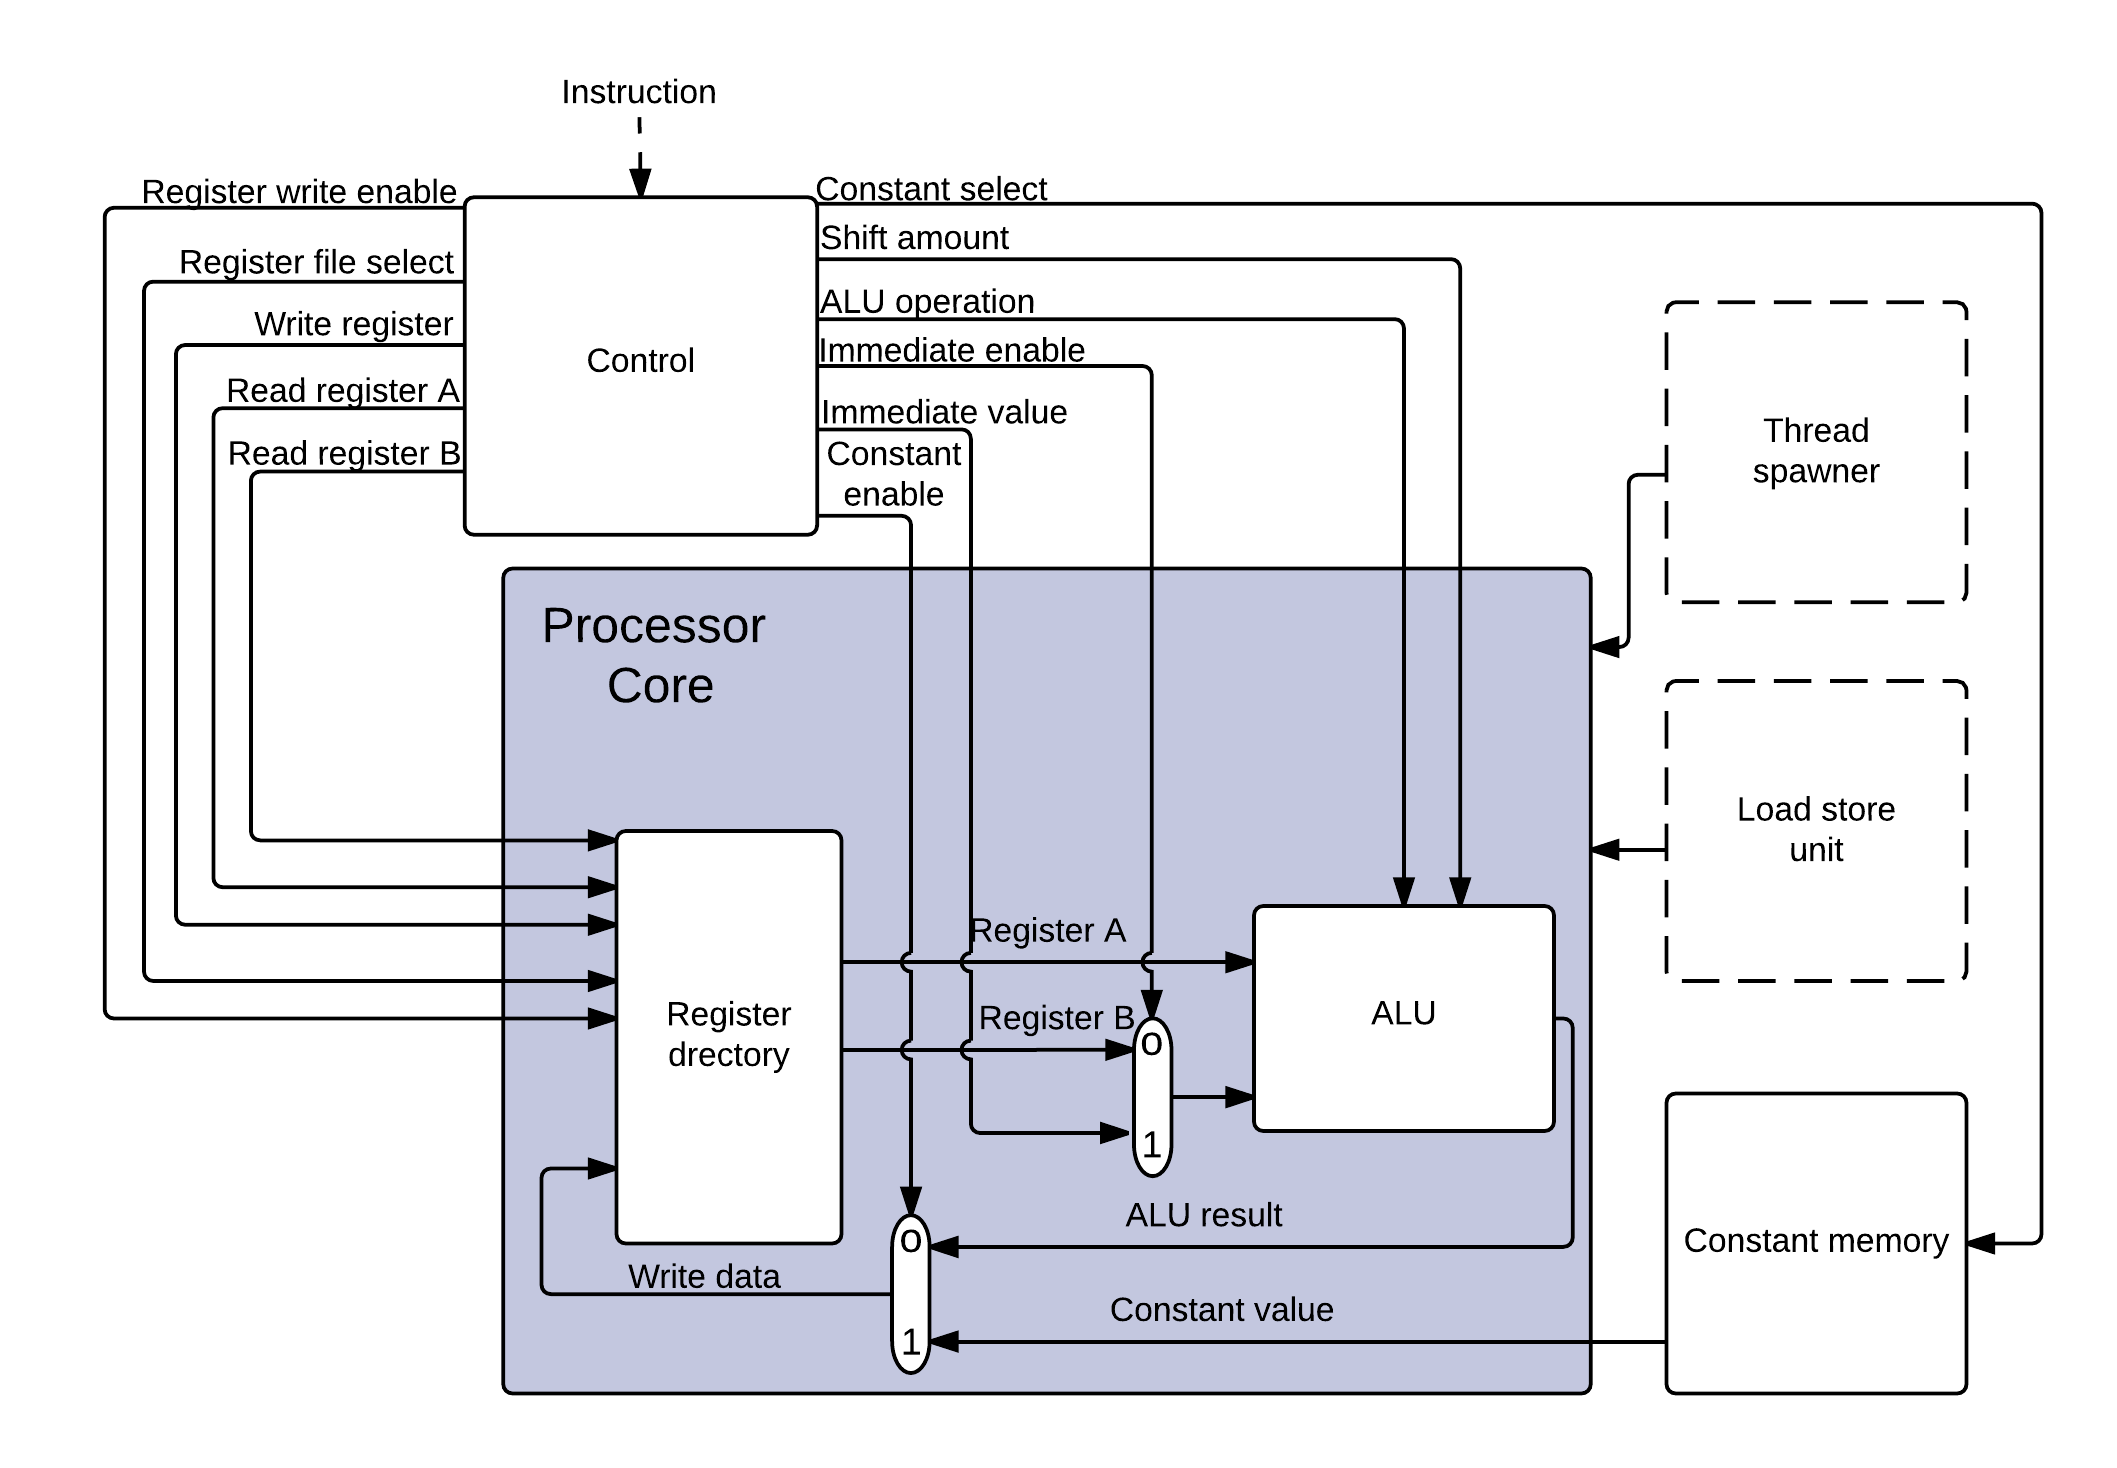
\includegraphics[width=1.2\textwidth]{../gpu/diagrams/processor_core.png}
	\caption{A single processor core.}
	\label{fig:processor_core}
\end{figure}

Each processor core contains an ALU and a register directory.
On each clock cycle the ALU receives the selected values from the register directory.
On the same cycle, the value is written back to the register selected by the control unit.

If the current instruction is a \emph{load constant} instruction, the control unit selects which constant to fetch from constant memory.
The constant enable signal is asserted, causing the multiplexer to select the constant value as the write back value.
The constant memory is stored on chip, meaning it returns the constant on the same cycle as it is requested.

To perform immediate instructions, the control unit asserts the \emph{immediate enable} signal.
The immediate value is then selected by the multiplexer and used as an operand in the ALU.

The architecture contains multiple processor cores like the one in figure \ref{fig:processor_core}.
Each of the cores receive the same control signals for the instructions.